\documentclass[9pt,twocolumn,twoside]{../../styles/osajnl}
\usepackage{fancyvrb}
\journal{i524} 

\title{Neo4J}

\author[1]{Sowmya Ravi}


\affil[1]{School of Informatics and Computing, Bloomington, IN 47408, U.S.A.}

\affil[*]{Corresponding authors: sowravi@iu.edu.com}

\dates{project-000, \today}

\ociscodes{Cloud, I524}

% replace this with your url in github/gitlab
\doi{\url{https://github.com/cloudmesh/classes/blob/master/docs/source/format/report/report.pdf}}


\begin{abstract}
Neo4J is a graph database designed for fast data access and management. The data is stored in the form of nodes and relationships in Neo4J. The unique approach it takes to store data makes it an efficientent to store data that contain a large the number of relationships. Moreover, it has the ability to store trillions of data entries in a compact manner. Neo4J comes along with Cypher, a highly readable querying language. Neo4j achieves the high efficiency and throughput by distributed computing. The various modes of clustering in Neo4j renders the capability of distributed computing. This paper focuses elaborates on the architecture of Neo4j and its uses ~\cite{www-neo4j-intro}.  

\end{abstract}

\setboolean{displaycopyright}{true}

\begin{document}

\maketitle

\section{Introduction}
Certain problems present in the world cannot be solved by using relational databases. For e.g. a social graph representing the network of friends in a social networking website. In this case the number of relationships in the data is too extensive and the relational databases perform poorly. Graph data bases on the other hand make the task of storing large amounts of data relatively simple and efficient. Neo4J is one such NoSQL, graph database which was developed to be used in the kind of problems mentioned before~\cite{www-neo4j-intro2}.

Neo4j is an open source data management software. At its core, Neo4j stores data in the form of nodes and relationships. It is often deployed in a production environment as a fault tolerant cluster of machines. The high scalability and fast traversal times make it far more efficient than the conventional relational databases ~\cite{www-neo4j-intro}. 

\section{Cypher programing language}
Neo4j uses its own programming language, 
Cypher, for data creation as well as querying. Cypher is capable of doing SQL like actions. In addition, it can specifically perform a powerful query called traversals. Traversal involves moving along a specific set of nodes in the database thereby tracing a path. This allows to leverage the spatial structuring of the data to get valuable information, similar to network 
analysis ~\cite{www-slideshare}. 

\section{Clustering }
This section discusses Neo4js architecture with respect to clustering. Clustering is the process of grouing instances or items. In the context of Neo4j, a number of maches are clustered in a group. The machines are connected and can communicate with one another. Each machine can be visulaized as a separate node in the cluster which performs a part or whole of the task assigned by a process to Neo4j. Neo4j uses clustering of machines to achieve high throughput, availability and disaster recovery~\cite{www-neo4j}. Neo4j offers two kind of clustering 
\begin{enumerate}
    \item Causal Clustering
    \item Highly Available clustering
\end{enumerate}
Each type of cluster has a unique set of features. The mode of clustering is chosen according to the application and requirements. 
\subsection{Causal Clustering}
The Causal clustering of machines in Neo4j is aimed at providing two important features: safety and scalability. ~\cite{www-neo4j-causal}

\begin{figure}[htbp]
\centering
\fbox{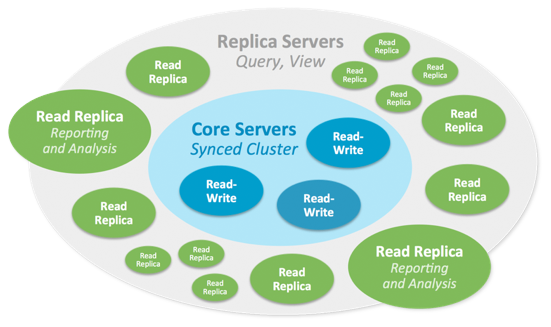
\includegraphics[width=\linewidth]{images/causal-clustering}}
\caption{Architecture of Causal Clustering ~\cite{www-neo4j-causal}}
\label{fig:false-color}
\end{figure}

 For operational purposes, the cluster is usually separated into two components: the core servers and the read replicas. The architecture of causal clustering is shown in Fig.2. All the write operations coming from the app servers are performed by the core servers while data is read by the app servers from the read replicas. The following sub-sections datail the wrorking of core servers and read replicas and also how they ensure safe and scalable data storage. 
\subsubsection{Core Servers}. 
The Core servers are responsible for safe data storage. This is achieved by replicating all incoming queries/transactions using Raft protocol (A log replication protocol)~\cite{www-neo4j-causal}. The protocol ensures the durability of data before committing to the query request. Usually, a transaction is accepted only when a majority of the servers,calculated as $N+1/2$ , have accepted it. This number is directly proportional to the number of core servers $N$. Hence, as the number of core servers grows, the size of majority required for committing to an end user also increases~\cite{www-neo4j-causal}. 

In practice, few machines in the core server cluster is enough to provide fault tolerance. This number is calculated using the formula: $N = 2F +1 $ where $N$ is the number of servers required to tolerate $F$ faults~\cite{www-neo4j-causal}. When a core server suffers a large number of faults, it is automatically converted to a read-only server for safety purposes. 

\subsubsection{Read replicas}
Read Replicas are Neo4j databases that scale out the incoming queries and procedures. They act like cache memories to the core servers which safeguard the data. Even though the read replicas are full-fledged databases, they are equipped to perform arbitrary read-only activities~\cite{www-neo4j-causal}.

Read Replicas are created asynchronously by core servers through log-shipping~\cite{www-neo4j-causal}. Log shipping occurs when the read replicas poll the core servers for new transactions and the transactions are shipped from the core severs to the read replicas. This polling occurs periodically. Usually, a small number of core servers ship out queries to a relatively large number of read replicas, allowing a large fan out of workload thereby, achieving scalability~\cite{www-neo4j-causal}. The read replicas unlike the core servers do not participate in deciding the cluster topology. 

\subsubsection{Causal Consistency}
In applications, data is generally read from a graph and written to a graph. In order to ensure the causal consistency in the data, the write operation must take into account previous write operations. The Causal Consistency model for distributed computing requires every node in the system to see causally related operations in the same order. This model ensures that the data can be written to cores and the written data be read from read replicas.
Fig.3 illustrates a Causal Cluster with causal consistency

\begin{figure}[htbp]
\centering
\fbox{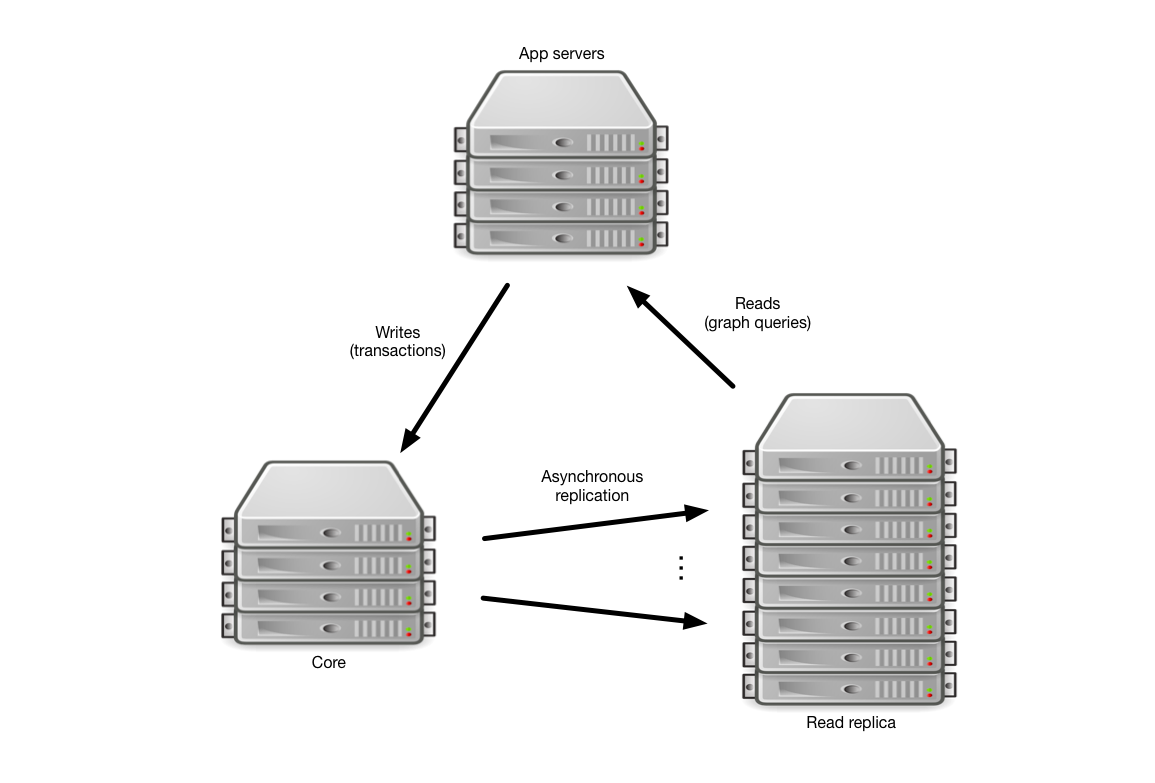
\includegraphics[width=\linewidth]{images/causal-clustering-drivers}}
\caption{Causal Cluster with causal consistency set via Neo4j drivers ~\cite{www-neo4j-causal}}
\label{fig:false-color}
\end{figure}

\section{Highly Available cluster}
The causal cluster discussed in the previous section focuses on safety and security. There is a division of work between the core servers and read replicas in the causal cluster. The Highly available cluster however, ensures continuous availablity. In this type of cluster each instance of the cluster contains full copy of the data in their local database. Thus each instance in the cluster is fully capable of performing all operations thereby achieving high availability. The cluster can be visualized as containing a single master with multiple slaves in which each instance is connected to every other instance(A 3 member cluster is shown in Fig.4)

\begin{figure}[htbp]
\centering
\fbox{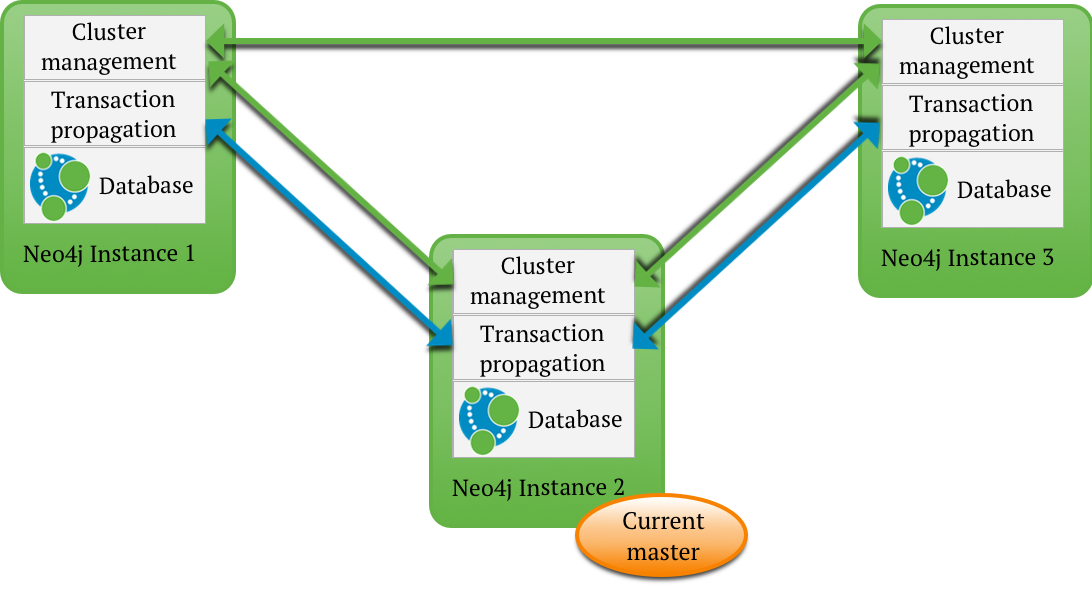
\includegraphics[width=\linewidth]{images/ha-architecture-neo-styled}}
\caption{A Highly Available cluster model~\cite{www-neo4j-ha}}
\label{fig:false-color}
\end{figure}

Also, each instance contains the logic to perform read/write operations and election management~\cite{www-neo4j-ha}. Every slave, excluding the Arbiter instance periodically communicate with the master to keep databases up to date~\cite{www-neo4j-ha}. There is a special slave called the Arbiter explained in the following section.
\subsubsection{Arbiter Instance}
The Arbiter instance is a special slave  that participates in cluster management activities but does not contain any replicated data. It simply contains a Neo4j software running in arbiter mode~\cite{www-neo4j-ha}. 
\subsubsection{Transaction Propagation}
Write Transactions performed directly on the Master will be pushed to slaves once the transaction is successful. When a write transaction is performed on a slave, the slave synchronizes with the Master after each write operation. The write operation on slave is always performed after ensuring that the slave is synchronized with the Master~\cite{www-neo4j-ha}.  

\section{Use Cases}
Neo4j can be used for fraud detection, network and IT operations, Real-time recommendation system, Social Network and Identity and Access Management~\cite{www-neo4j-uc}. A sample use case in fraud detection is described below. 

\subsubsection{Neo4j for First Party Fraud  Detection}
First party fraud occurs when a person uses illegitimate information to secure credit card. Often two or more people share certain information to create multiple identities and operate as a ring.  Neo4j is a great tool to detect fraud rings. In Neo4j, all the customer related data is stored as a directed graph. When more than two people share the same contact information like address or SSN and have outstanding loans or credit, this may potentially be a fraud ring. It is possible to discover similar connections by writing simple queries in Cypher. In relational Databases, this network is present in tables with rows and columns. Complex joins have to performed to find a fraud ring and joins are expensive operations. Moreover, in real-time analysis scalability could be a serious issue. Neo4j achieves scalability when operated in a causal clustering mode. The simplicity and robustness of Neo4j makes it a great tool for fraud detection~\cite{gorkasadowksi&philiprathle2015}.

\section{Conclusion}
Neo4j being an open source, graph based and a highly scalable software, it is suitable for applications that deal with data containing numerous relationships. It offers two different clustering modes it can operate in, each focusing on a certain feature. In addition, Cypher the query language is very simple and finds relationships without performing costly operations like joins. The simplicity and  versatility of Neo4j makes it a great software aid for data scientists trying to analyze relationships and networks in real time as well as in batch. 

% Bibliography

\bibliography{references}
 
\section*{Author Biographies}
\begingroup
\setlength\intextsep{0pt}
\begin{minipage}[t][3.2cm][t]{1.0\columnwidth} % Adjust height [3.2cm] as required for separation of bio photos.
  \begin{wrapfigure}{L}{0.25\columnwidth}
    
\includegraphics[width=0.25\columnwidth]{images/john_smith.eps}
  \end{wrapfigure}
  \noindent
  {\bfseries Sowmya Ravi} pursuing Masters in Data Science from Indiana University. Her research interests include Machine Learning, Data Mining and Big Data Analytics
\end{minipage}

\endgroup

\newpage

\appendix



\end{document}
